\documentclass{scrartcl}

\usepackage[utf8]{inputenc}
\usepackage[T1]{fontenc}
\usepackage[ngerman]{babel}
\usepackage{amssymb}
\usepackage{amsmath}
\usepackage{graphicx}
\usepackage{framed}
\usepackage{xcolor}
\usepackage[nottoc]{tocbibind}
\usepackage{caption}

\colorlet{shadecolor}{gray!25}
\setlength{\parindent}{0pt}

\newcommand{\abs}[1]{\left\lvert#1\right\rvert}


\begin{document}

\title{Lösen des Poisson-Problems mittels Finite-Differenzen-Diskretisierung\\
und CG-Verfahren}
\author{Marisa Breßler und Anne Jeschke (PPI27)}
\date{07.02.2020}
\maketitle

\tableofcontents

\pagebreak
\section{Motivation}
In unserem vorherigen Berichten haben wir das Poisson-Problem vorgestellt und einen numerischen Lösungsansatz aufgezeigt, der es durch eine Diskretisierung des Gebietes und des Laplace-Operators in das Lösen eines linearen Gleichungssystems überführt.
Die dabei entstehende tridiagonale Blockmatrix ist dünn besetzt, d.h. nur wenige Einträge sind ungleich Null.
Deswegen ist es sinnvoll, sie als sogenannte \textit{sparse}-Matrix abzuspeichern.
Dieser Speicherplatzvorteil geht jedoch beim Lösen des linearen Gleichungssystems mittels Gauß-Algorithmus und LU-Zerlegung verloren, da eine LU-Zerlegung einer dünn besetzten Matrix im Allgemeinen nicht dünn besetzt ist.
Aufgrund dieses Umstandes erscheint es sinnvoll, das lineare Gleichungssystem nicht direkt, sondern iterativ zu lösen.
Solche iterativen Lösungsverfahren (wie das Gesamtschrittverfahren von Jacobi, das Einzelschrittverfahren von Gauß-Seidel, das SOR-Verfahren und das CG-Verfahren) bieten gegenüber direkten Verfahren außerdem den Vorteil, dass deren Rechenaufwand im Verhältnis zur in der Praxis für gewöhnlich sehr großen Dimension der Blockmatrix recht gering ist.
Da das CG-Verfahrens eine heute durchaus übliche Methode zum Lösen großer linearer Gleichungssysteme darstellt, wollen wir dieses im Folgenden im Rahmen unseres bisherigen Settings (Poisson-Problem und Finite-Differenzen-Diskretisierung) vorstellen und untersuchen.



\pagebreak
\section{Theoretische Grundlagen und Algorithmus}
iterative Verfahren bestimmen Näherungslösung, via Grenzwert an exakte Lösung \\
\\
für CG-Verfahren muss Matrix symmetrisch positiv definit sein \\
ist für unsere Blockmatrix der Fall, da sie symmetrisch ist, positive Diagonalelemente besitzt und irreduzibel diagonaldominant ist (> positiv definit) \\
\\
während sich die anderen oben genannten iterativen Verfahren die Methode des Splitting zunutze machen, ist die Idee des CG-Verfahrens die folgende: \\
Lösung des linearen Gleichungssystems in ein Minimierungsproblem überführen \\
dazu wird folgende Funktion definiert: ... \\
diese hat genau an der Stelle $x$ ihr einziges Minimum, wo auch das LGS $Ax=b$ seine Lösung hat \\
man konstruiert Abstiegsrichtungen so ..., dass Funktionswerte immer kleiner werden \\
...

\pagebreak
\section{Experimente und Beobachtungen}

\subsection{Entwicklung des absoluten Fehlers der Iterierten}
{
  \centering
    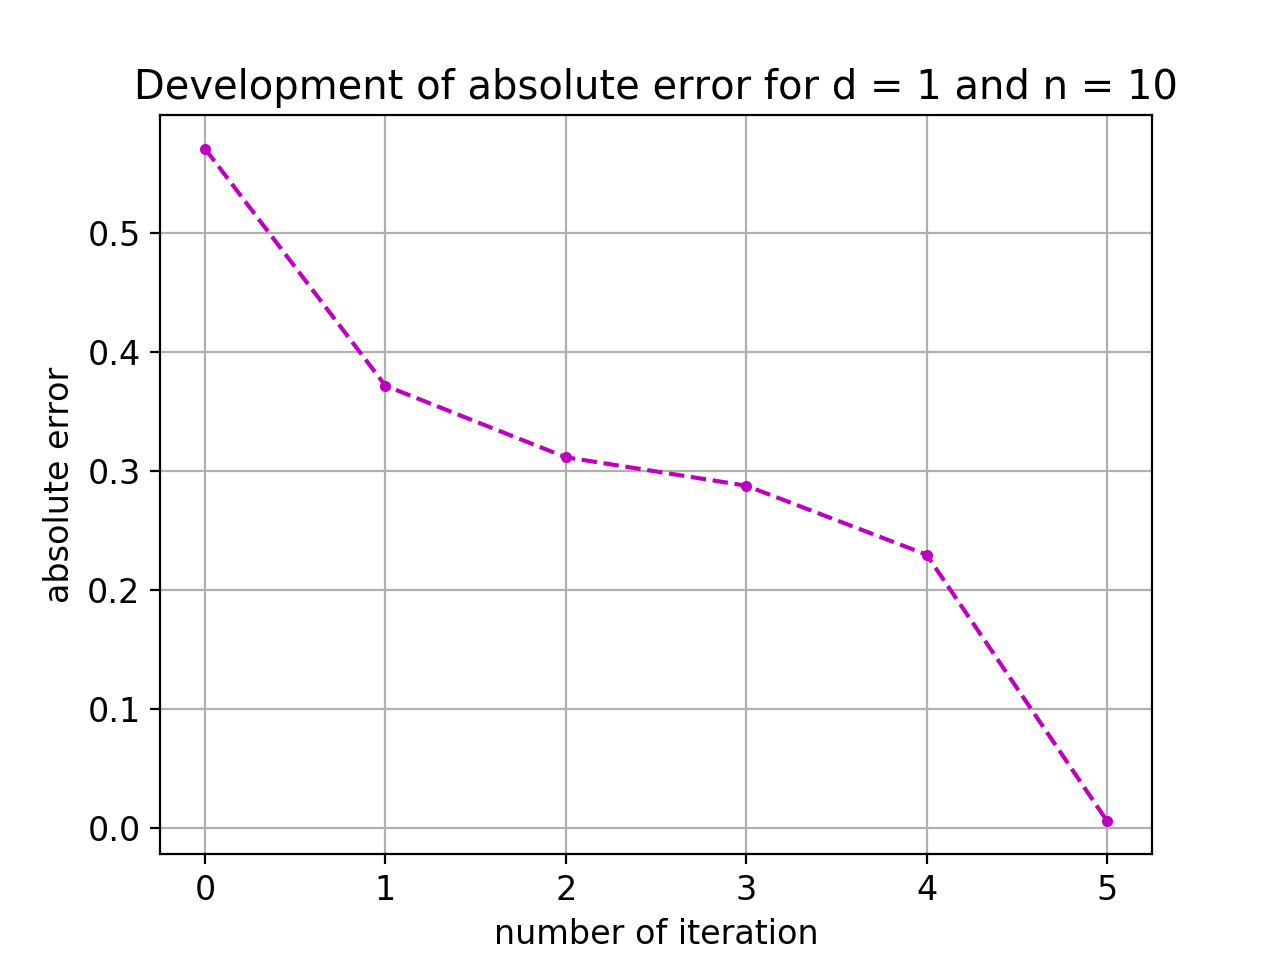
\includegraphics[width=0.45\textwidth]{Grafiken/iterates_d1_n10}
    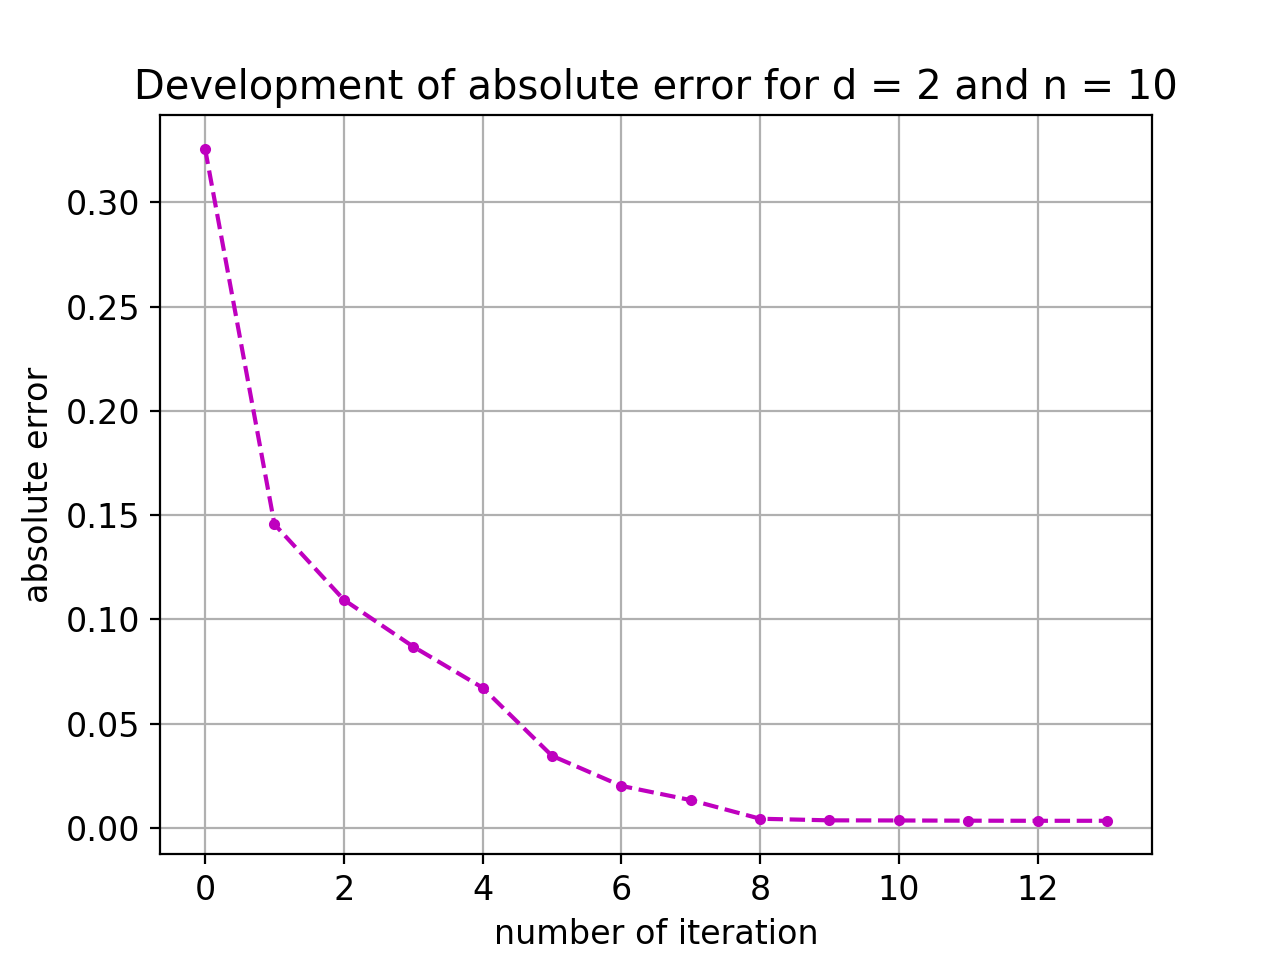
\includegraphics[width=0.45\textwidth]{Grafiken/iterates_d2_n10}
    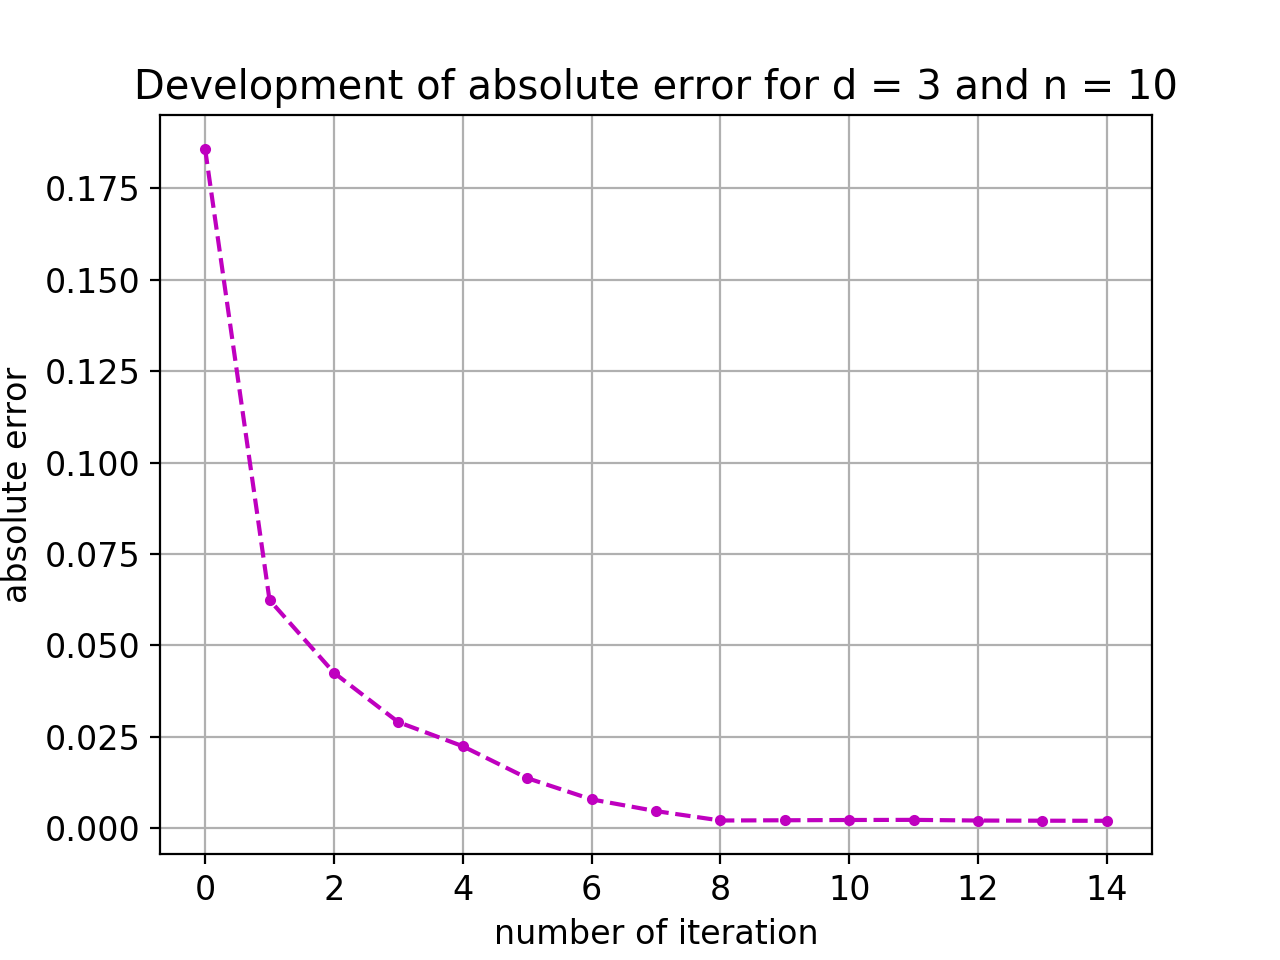
\includegraphics[width=0.45\textwidth]{Grafiken/iterates_d3_n10}
    \vspace{-0.2cm}
    \captionof{figure}{Entwicklung des Fehlers pro Iteration für $d\in\{1, 2, 3\}$ und $n=10$}
}
\vspace{0.5cm}

\pagebreak
\subsection{Konvergenzverhalten für ein festes Epsilon}
{
  \centering
    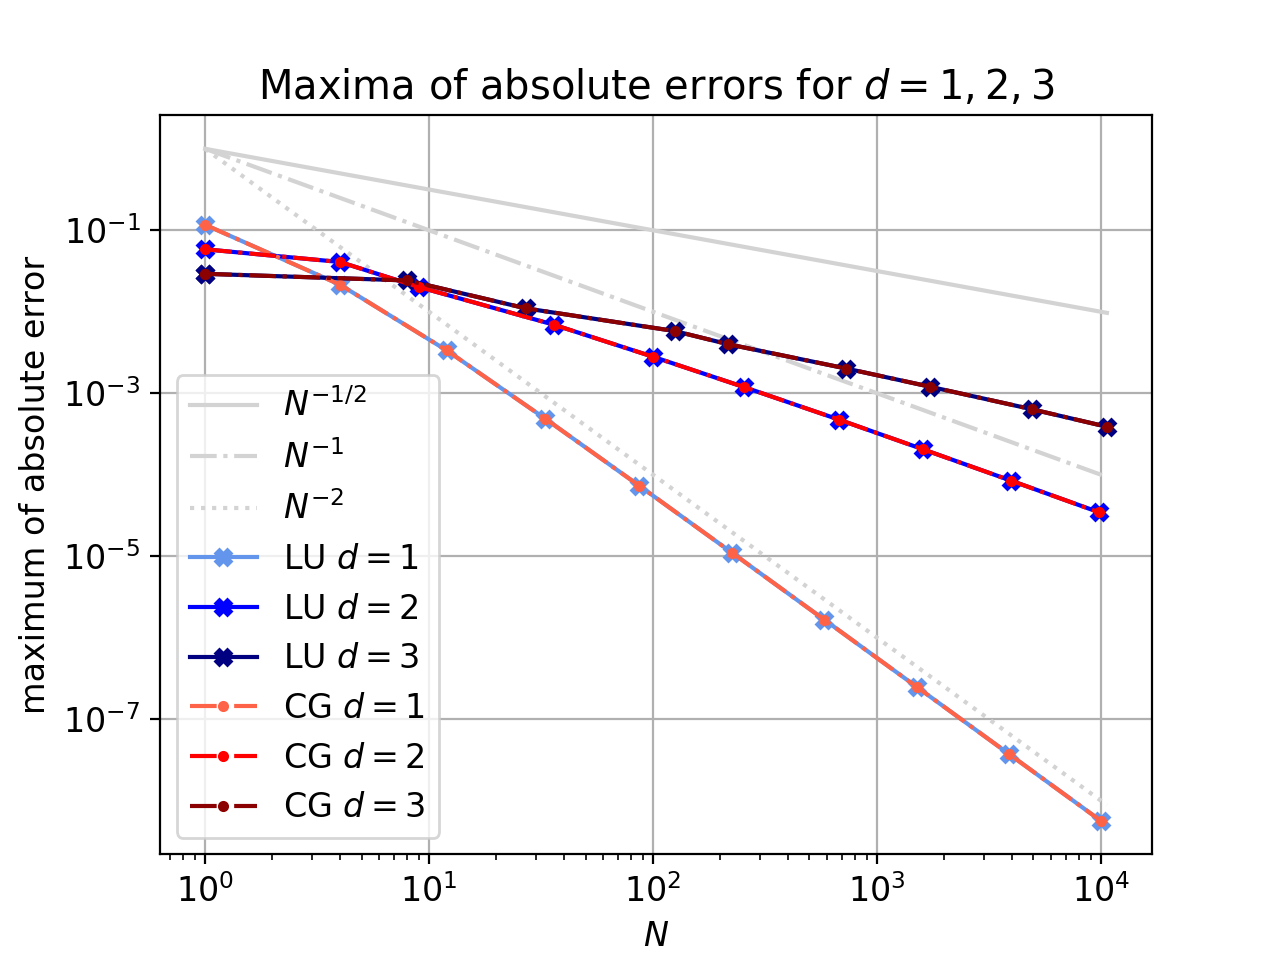
\includegraphics[width=0.75\textwidth]{Grafiken/compare}
    \vspace{-0.2cm}
    \captionof{figure}{Konvergenzverhalten für $\epsilon = 10^{-8}$ für $d\in\{1, 2, 3\}$ im Vergleich zur LU Zerlegung}
}
\vspace{0.5cm}

Konvergenz abh. von Diskretisierung, nicht von Lösungsverfahren

\pagebreak
\subsection{Konvergenzverhalten für variable Epsilon}
{
  \centering
    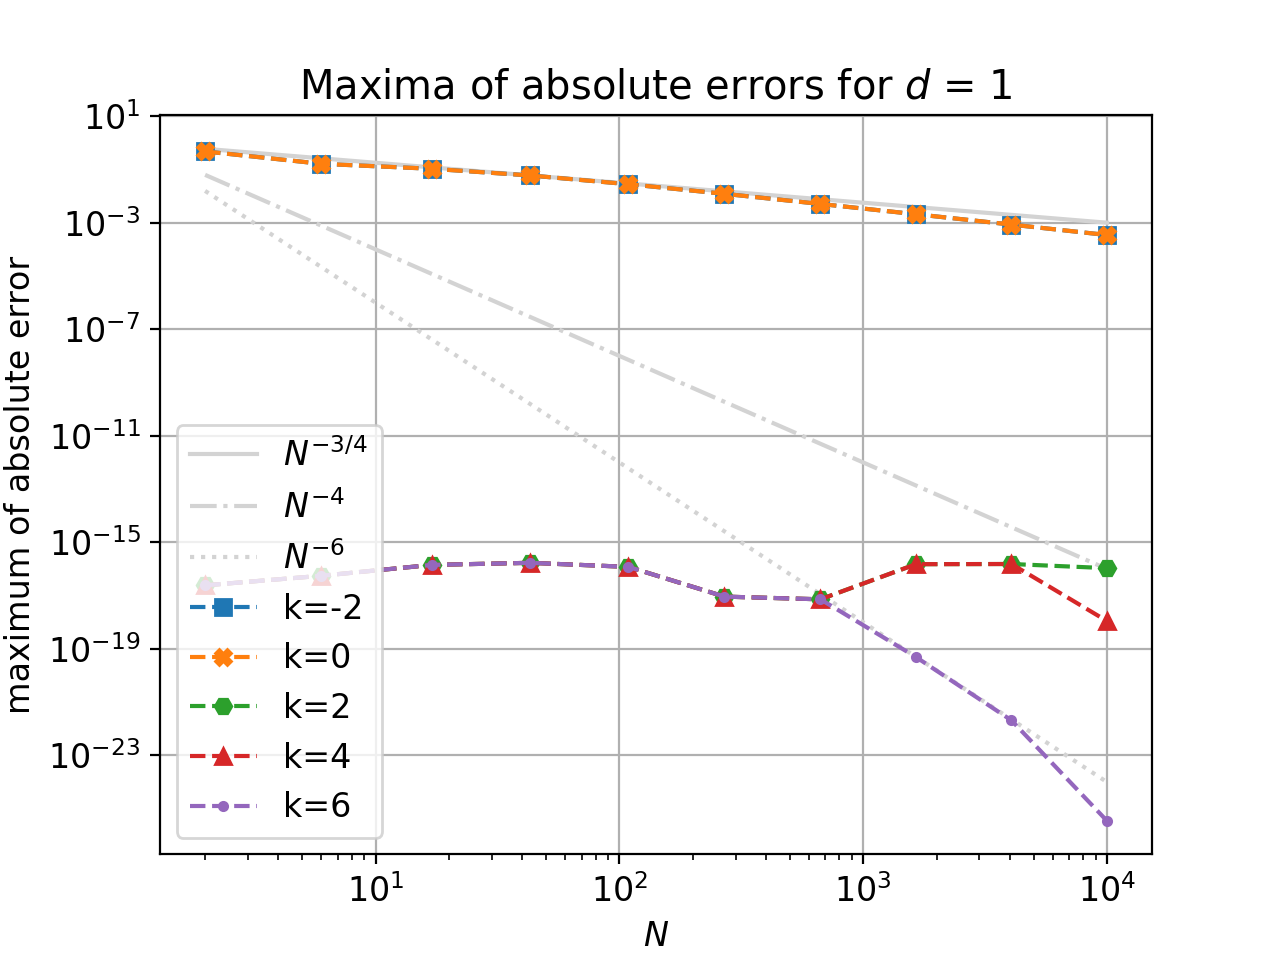
\includegraphics[width=0.45\textwidth]{Grafiken/epsilon_d1}
    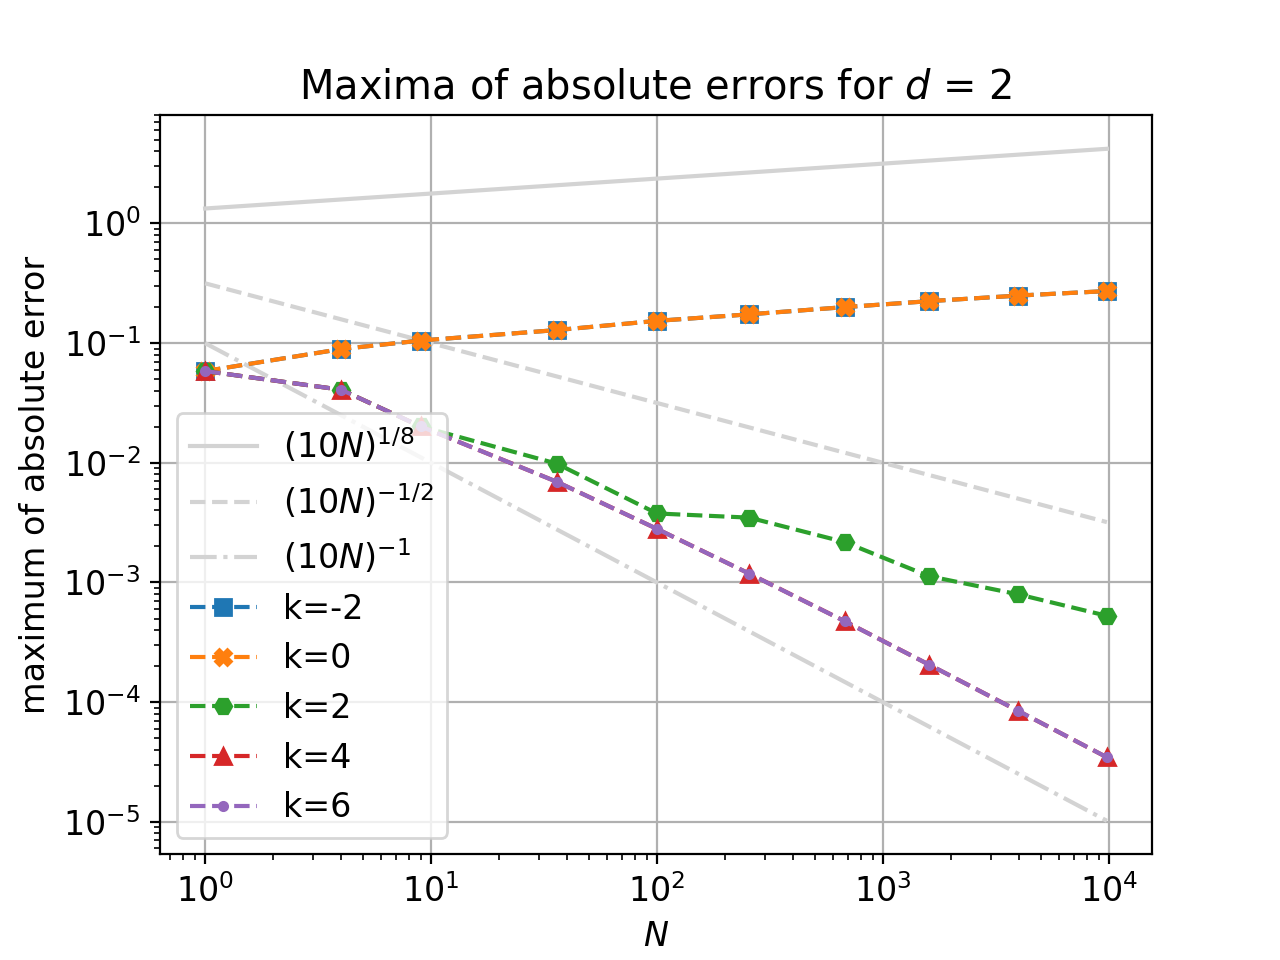
\includegraphics[width=0.45\textwidth]{Grafiken/epsilon_d2}
    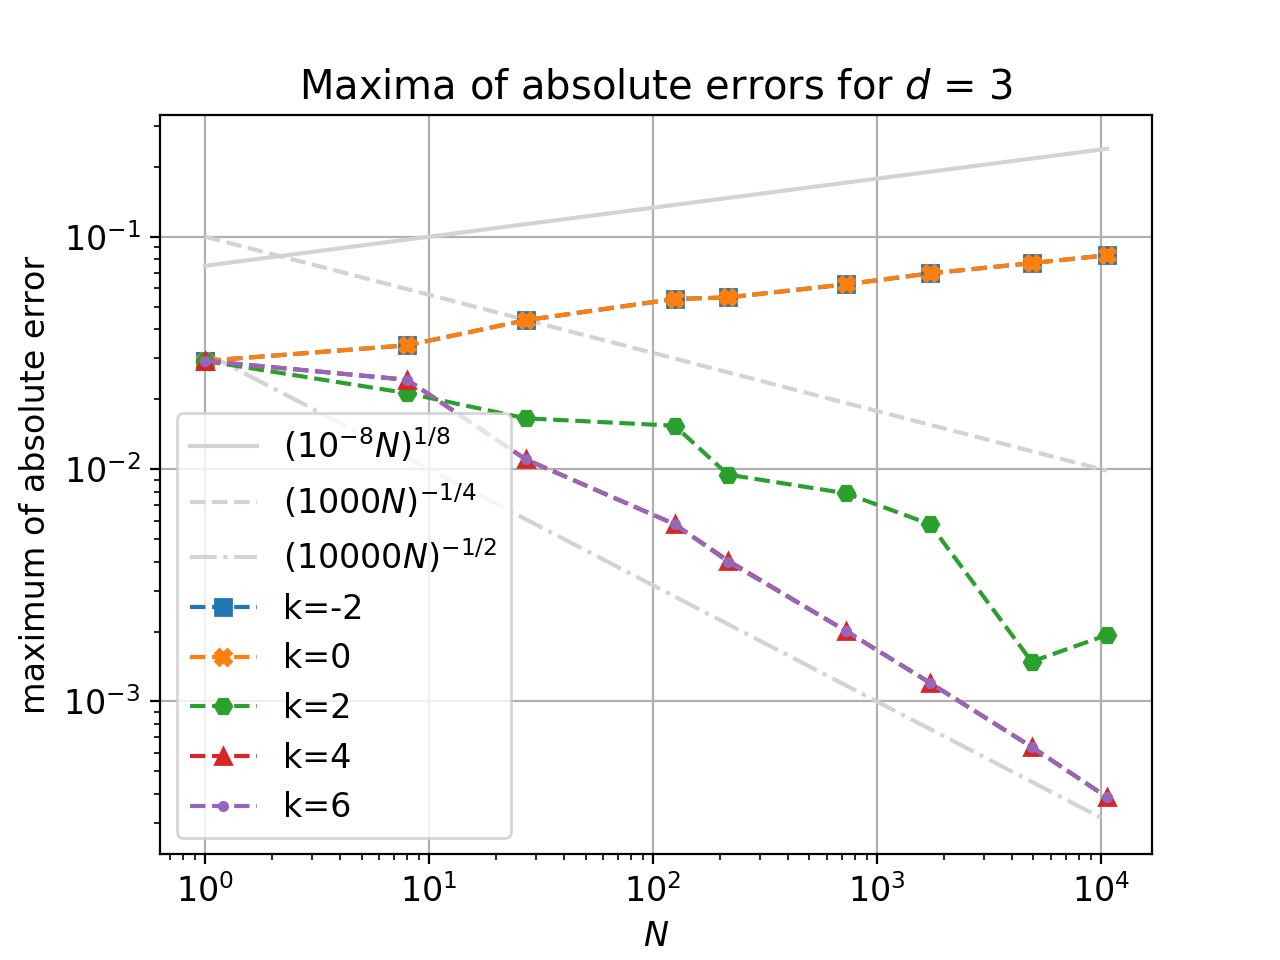
\includegraphics[width=0.45\textwidth]{Grafiken/epsilon_d3}
    \vspace{-0.2cm}
    \captionof{figure}{Konvergenzverhalten für $\epsilon^{(k)}=n^{-k}$ für $d\in\{1, 2, 3\}$}
}
\vspace{0.5cm}

- 0, -2 gleich

\pagebreak
\section{Abschließende Worte}



\end{document}
